\documentclass[a4j]{jarticle}
\usepackage{amsmath} % 数式用
\usepackage[dvipdfmx]{graphicx} % 画像用
\usepackage{geometry} % 余白設定用
\usepackage{float} % 図表の位置調整用

\geometry{left=25mm, right=25mm, top=25mm, bottom=25mm} % 余白の設定

\begin{document}

\title{曲げ試験レポート}
\author{大阪大学 工学部 地球総合工学科 船舶海洋工学コース \\ 古賀光一朗}
\date{\today}
\maketitle

\section{目的}
三点曲げ実験を行い、ヤング率の計測、荷重とたわみ・荷重とひずみの関係について理論式との比較を通して、梁のたわみ挙動について理解を深める。さらに、自由振動実験を行い、振動の固有周波数と減衰係数の推定方法を習得する。

\section{実験の概要, 理論}
\subsection{使用機器}
本実験では、以下の主要な機器を使用した。
\begin{itemize}
    \item ひずみゲージ
    \begin{itemize}
        \item 梁の表面に貼付したひずみゲージを用いて、材料内部のひずみ状態を電気的に計測した。複数のひずみゲージを設置し、梁の長さ方向のひずみ分布も把握できるよう工夫した。
    \end{itemize}
    \item ダイヤルゲージ
    \begin{itemize}
        \item 梁中央部のたわみを高精度で計測するために使用した。
    \end{itemize}
    \item ノギス
    \begin{itemize}
        \item 梁の断面寸法(幅、高さ)および支点間距離を精密に計測するために使用した。
    \end{itemize}
    \item メジャー
    \begin{itemize}
        \item 梁の長さを計測するために用いた
    \end{itemize}
    \item 錘
    \begin{itemize}
        \item 段階的な荷重負荷に用いるため、個々の錘の正確な重量を事前に計測した。
    \end{itemize}
\end{itemize}

\subsection{実験手順}

本実験は、以下の手順で実施した。

\begin{enumerate}
    \item \textbf{寸法計測と設置}
    \begin{itemize}
        \item 試験に供する梁の幅, 厚さ, 長さをノギスとメジャーで正確に計測・記録した。
    \end{itemize}

    \item \textbf{錘の重量計測}
    \begin{itemize}
        \item 実験に使用する全ての錘の正確な重量を計測し、記録した。
    \end{itemize}

    \item \textbf{静的曲げ試験(荷重負荷と除荷)}
    \begin{itemize}
        \item 梁の中央部に段階的に錘を負荷し、それぞれの荷重ステップにおいて梁中央部のたわみと、複数の位置に設置されたひずみゲージによるひずみを同時に計測した。また、荷重を徐々に減少させる除荷プロセスも行い、材料の弾性挙動を確認した。
    \end{itemize}
    
    \item \textbf{動的試験(自由振動計測)}
    \begin{itemize}
        \item 全ての錘を梁に載せた状態で、梁中央部に瞬間的な衝撃を与えた。衝撃後の\textbf{自由振動時のたわみとひずみ}の時間応答を高速($100\,\mathrm{Hz}$)でサンプリングし記録した。
    \end{itemize}

    \item \textbf{グラフ作成}
    \begin{itemize}
        \item 取得した荷重、たわみ、ひずみのデータを用いて、それぞれ荷重-たわみ曲線および荷重-ひずみ曲線を作成した。
    \end{itemize}
\end{enumerate}

\subsection{三点曲げ}
三点曲げ試験は、\textbf{図\ref{fig:santenmage}}のように試験片を二点で支持し、その中央に荷重を加える試験である。

\begin{figure}[H]
\centering
    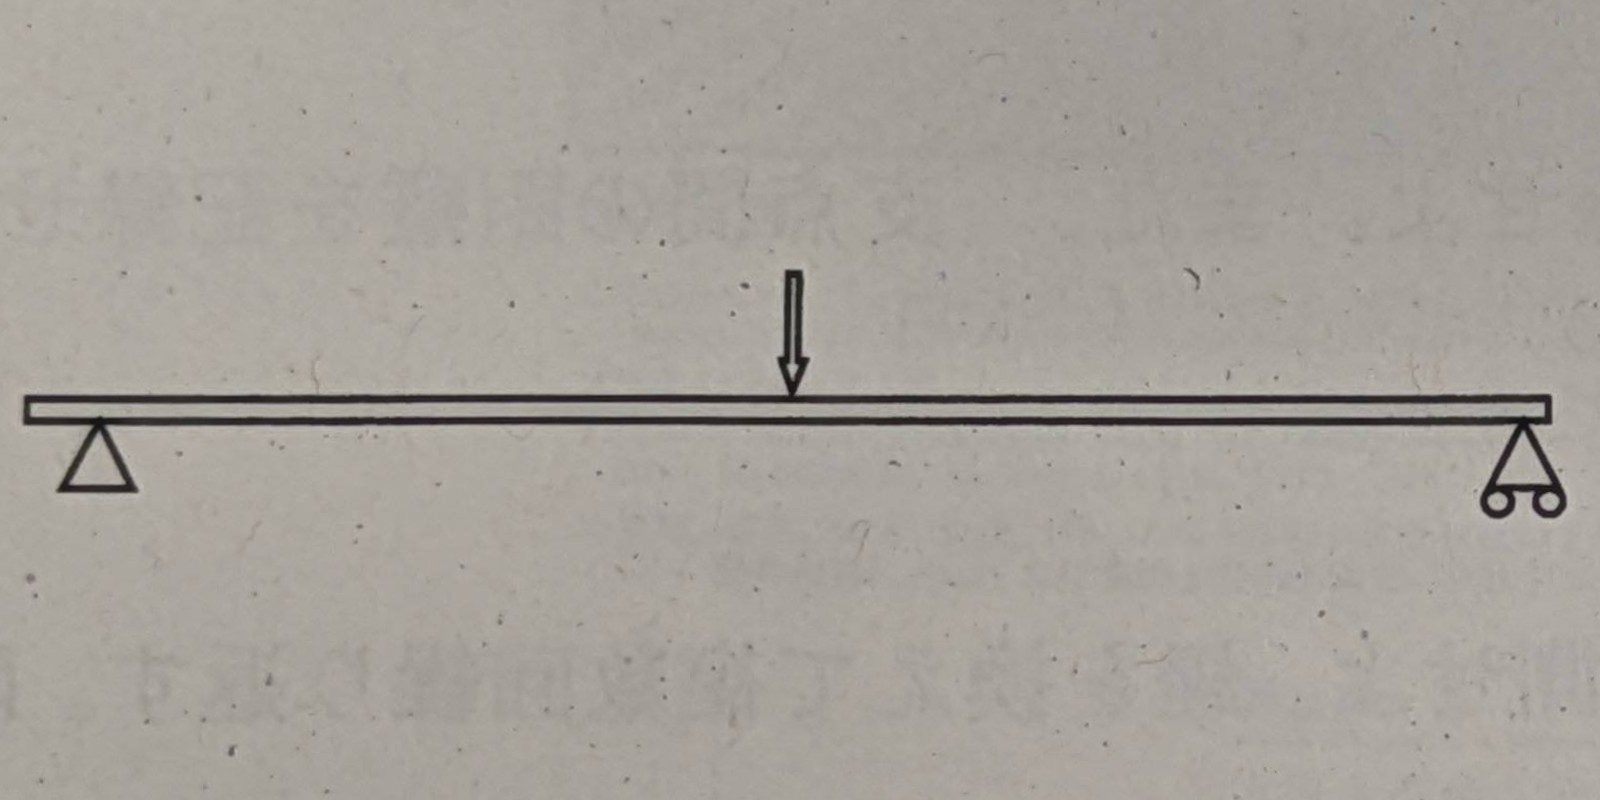
\includegraphics[width=0.8\textwidth]{summer/ship-experiment/bend/picture/santenmage.png}
    \caption{三点曲げ模式図}
    \label{fig:santenmage}
\end{figure}

このとき、せん断力図(SFD)と曲げモーメント図(BMD)は\textbf{図\ref{fig:sfd_bmd}}のようになる。

\begin{figure}[H]
    \centering
    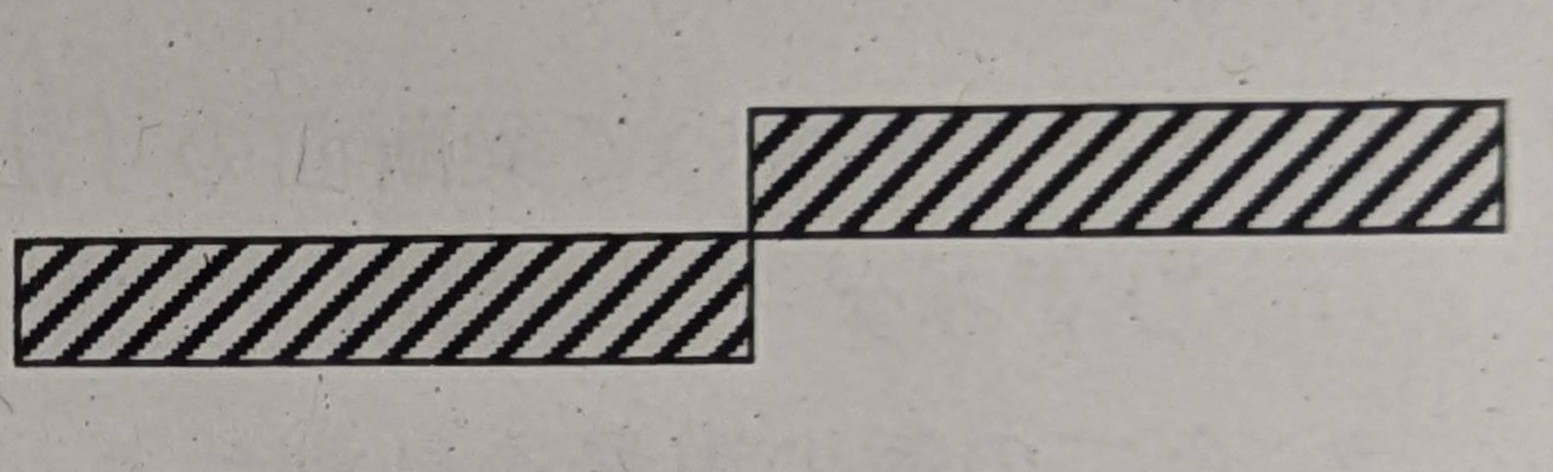
\includegraphics[width=0.5\linewidth]{summer/ship-experiment/bend/picture/sfd.png}
    \caption{三点曲げのせん断力図}
    \label{fig:sfd}
\end{figure}
\begin{figure}[H]
    \centering
    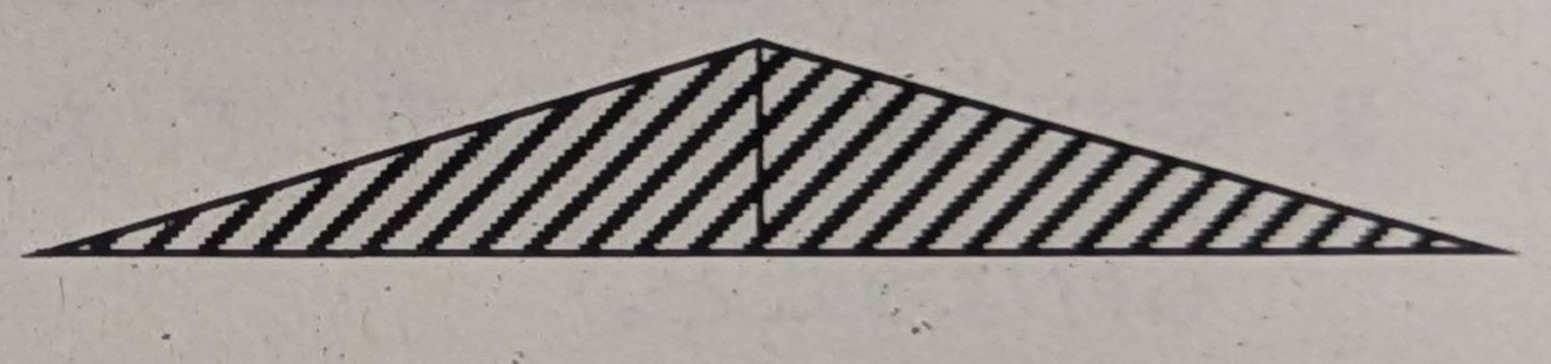
\includegraphics[width=0.5\linewidth]{summer/ship-experiment/bend/picture/bmd.png}
    \caption{三点曲げの曲げモーメント図}
    \label{fig:bmd}
\end{figure}


\subsection{三点曲げと変形の関係}
\label{sec:bending_theory}
梁の長さ$L$、ヤング率$E$、断面二次モーメント$I$とする。梁中央を原点($x=0$)として、たわみを$w(x)$とすると、曲げモーメント$M(x)$との間には以下の関係が成り立つ。
\begin{equation}
    EI\frac{d^2w}{dx^2} = M(x)
    \label{eq:beam_gov}
\end{equation}
三点曲げにおける曲げモーメント$M(x)$と、矩形断面の断面二次モーメント$I$は次式で与えられる。

\begin{align}
\label{eq:3point}
    M(x) &= \frac{P}{2} \left( \frac{L}{2} - |x| \right)\\
    I &= \frac{bh^3}{12}
\end{align}
ここで、$P$は中央の集中荷重、$b$は梁の幅、$h$は梁の厚さである。
支配方程式を支持点($x=\pm L/2$)でたわみとたわみ角が0になるという境界条件の下で解くと、たわみ$w$は次式で与えられる。
\begin{equation}
    w(x) = -\frac{P}{4EI} \left( \frac{L}{2}-x \right) \left[ -\frac{(\frac{L}{2}-x)^2}{3} + \frac{L^2}{4} \right]
    \label{eq:deflection}
\end{equation}
一方で梁の表面($z$方向の位置)のひずみ$\epsilon$は次式で表される。
\begin{equation}
    \epsilon = \frac{M(x)z}{EI}
    \label{eq:strain}
\end{equation}

\subsection{梁の自由振動}
減衰を考慮した1自由度の運動方程式は、質量$m$、ばね定数$k$、減衰比$\gamma$を用いて以下で記述される。
\begin{equation}
    m\ddot{w} + 2\gamma\sqrt{mk}\dot{w} + kw = 0
    \label{eq:free_vibration_gov}
\end{equation}
この運動方程式の解は、次式で与えられる。
\begin{equation}
    w(t) = e^{-\gamma\omega_{0}t} \left[ A\cos \left( \sqrt{1-\gamma^2}\omega_{0}t \right) + B\sin \left( \sqrt{1-\gamma^2}\omega_{0}t \right) \right]
    \label{eq:free_vibration_sol}
\end{equation}
ここで、$\omega_0 = \sqrt{k/m}$であり、$A, B$は初期条件で決まる定数である。この式から、振幅が時間と共に減衰していく様子がわかる。
実験データから減衰比$\gamma$を求めるには、隣り合う振動の振幅$A_i$と$A_{i+1}$の比(対数減衰率)を用いる。
$$
\gamma = \frac{1}{2\pi} \ln \left( \frac{A_i}{A_{i+1}} \right)
$$

\subsection{中央部に大質量を有する両端支持梁の固有周波数}
剛性$EI$、長さ$L$の両端支持梁の中央に荷重$P$が作用するときの変位量$\delta$は次式で与えられる。
\begin{equation}
    \delta = \frac{PL^3}{48EI}
    \label{eq:static_deflection_center}
\end{equation}
この式を$P$について解くと$P = (48EI/L^3)\delta$となり、$P=k\delta$の関係から、この梁の等価なばね定数$k$が求まる。
梁の中央に十分大きな質量$M$が取り付けられている場合、慣性力とばねによる復元力の釣り合いは、
\begin{equation}
    M\ddot{\delta} + k\delta = 0
    \label{eq:mass_beam_gov}
\end{equation}
という単振動の運動方程式で表せる。これより、系の固有角振動数$\omega$は次式となる。
\begin{equation}
    \omega = \sqrt{\frac{k}{M}} = \sqrt{\frac{48EI}{ML^3}}
    \label{eq:natural_freq}
\end{equation}


\section{結果}

\subsection{梁の寸法}
試験に用いた梁の寸法を測定した結果を\textbf{表\ref{tab:beam_dim}}に示す。
\begin{table}[H]
  \centering
  \caption{梁の寸法}
  \label{tab:beam_dim}
  \begin{tabular}{|l|c|c|c|c|}
    \hline
    測定箇所 & 1回目[mm] & 2回目[mm] & 3回目[mm] & 平均値[mm] \\ \hline
    幅 & 24.90 & 25.00 & 24.89 & 24.93 \\ \hline
    板厚 & 4.05 & 4.30 & 4.02 & 4.12 \\ \hline
    長さ & 811 & - & - & 811 \\ \hline
  \end{tabular}
\end{table}

\subsection{ひずみゲージの位置}
梁の中心を原点としたときの、各ひずみゲージのx座標を\textbf{表\ref{tab:gauge_pos}}に示す。
\begin{table}[H]
  \centering
  \caption{ひずみゲージの位置}
  \label{tab:gauge_pos}
  \begin{tabular}{|c|c|c|c|c|c|}
    \hline
    CH1 & CH2 & CH3 & CH4 & CH5 & CH6 (裏面) \\ \hline
    -300 & -200 & -100 & 10 & 200 & 10 \\ \hline
  \end{tabular}
  \\(単位: mm)
\end{table}

\subsection{錘の質量}
\label{tex:omori}
本実験の静的曲げ試験で用いた錘の質量を\textbf{表\ref{tab:weights}}に示す。
\begin{table}[H]
    \centering
    \caption{使用した錘の質量}
    \label{tab:weights}
    \begin{tabular}{|l|c|}
        \hline
        錘の種類 & 質量 [kg] \\ \hline
        錘A & 1.3155 \\ \hline
        錘B & 0.999 \\ \hline
        錘C & 0.1999 \\ \hline
    \end{tabular}
\end{table}

\subsection{静的過程}
\subsubsection{ひずみ-時間曲線, たわみ-時間曲線}
ひずみゲージから得られた生データをグラフにすると以下のような挙動が見られた
\begin{figure}[H]
    \centering
    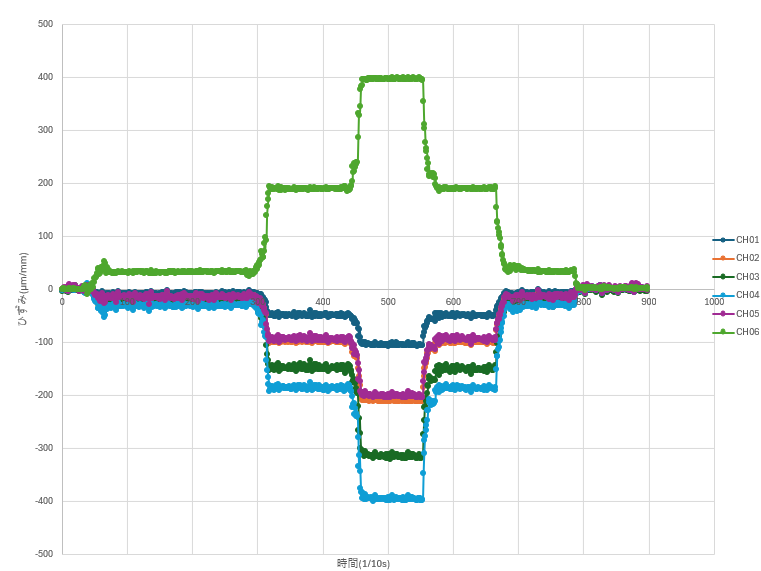
\includegraphics[width=0.8\linewidth]{summer/ship-experiment/bend/picture/hizumi-time.png}
    \caption{ひずみ-時間曲線}
    \label{fig:hizumi-time}
\end{figure}

また、ダイヤルゲージからのデータによると
\begin{figure}[H]
    \centering
    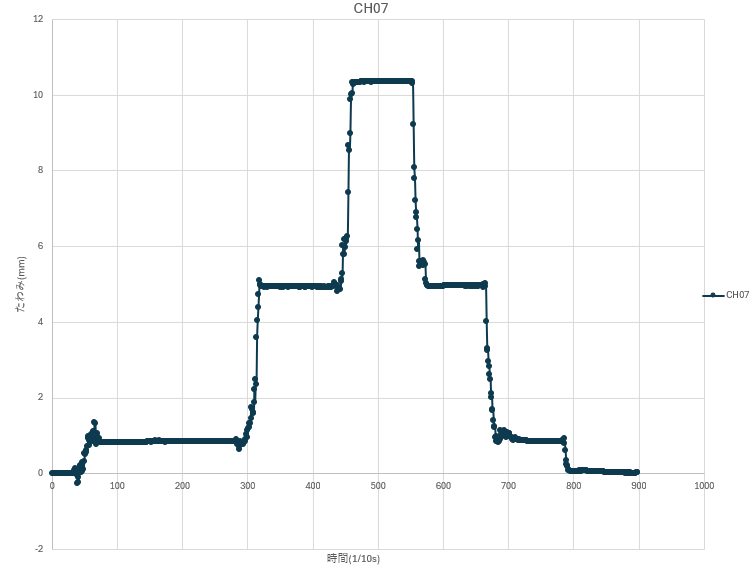
\includegraphics[width=0.8\linewidth]{summer/ship-experiment/bend/picture/tawami-time.png}
    \caption{たわみ-時間曲線}
    \label{fig:tawami-time}
\end{figure}

\subsubsection{荷重-ひずみ曲線}
縦軸に荷重 [N]、横軸にひずみ [µm/m] を取ったグラフ。
\begin{figure}[H]
    \centering
    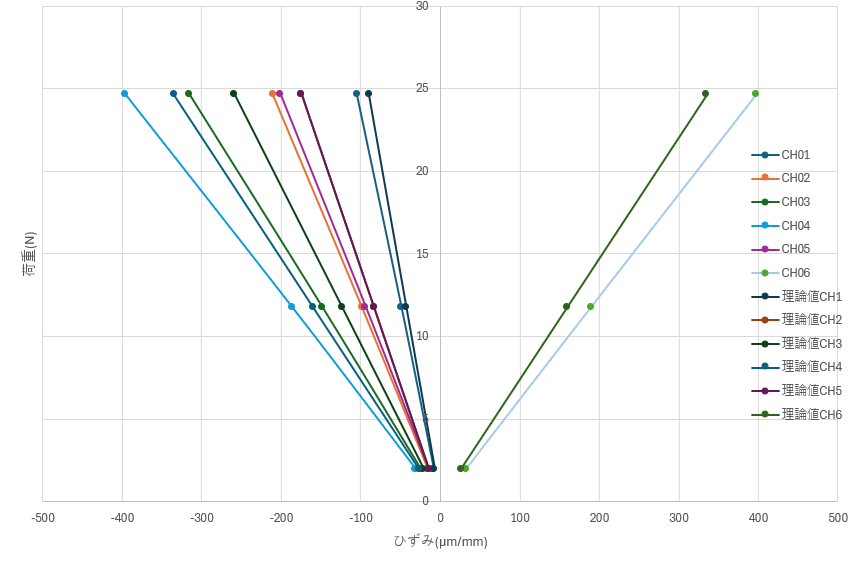
\includegraphics[width=0.8\linewidth]{summer/ship-experiment/bend/picture/kaju-hizumi.png}
    \caption{荷重-ひずみ曲線}
    \label{fig:kaju-hizumi}
\end{figure}

\subsubsection{荷重-たわみ曲線}
縦軸に荷重 [N]、横軸にたわみ [mm] を取ったグラフ。
\begin{figure}[H]
    \centering
    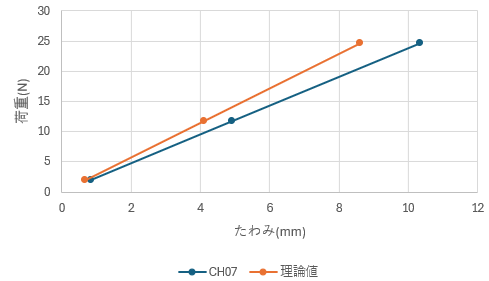
\includegraphics[width=0.8\linewidth]{summer/ship-experiment/bend/picture/kaju-tawami.png}
    \caption{荷重-たわみ曲線}
    \label{fig:kaju-tawami}
\end{figure}

\subsection{動的過程}
\subsubsection{ひずみ-時間曲線}
CH1~CH5のひずみゲージから得られた生データをグラフにすると以下のような挙動が見られた
\begin{figure}[H]
    \centering
    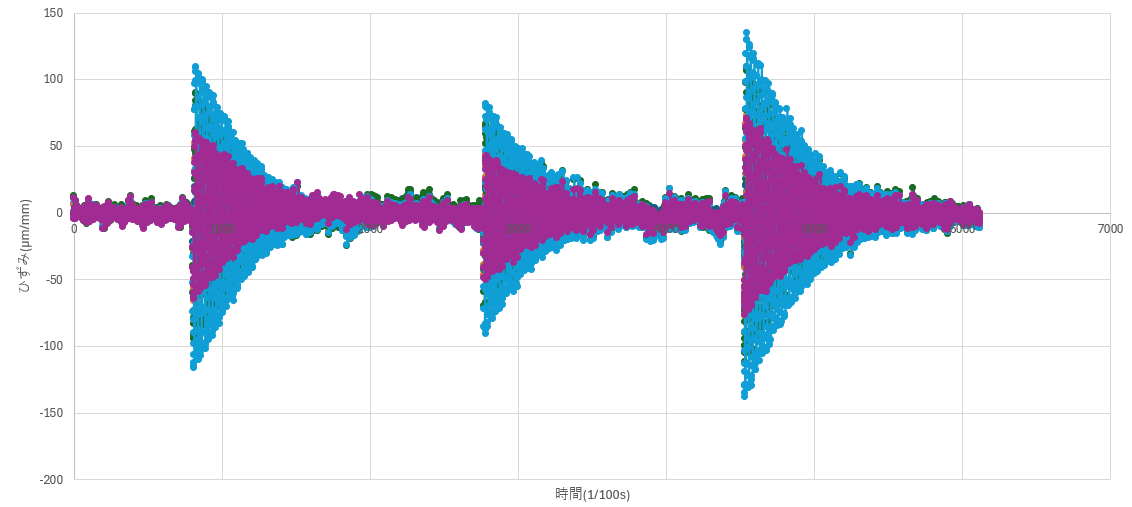
\includegraphics[width=0.8\linewidth]{summer/ship-experiment/bend/picture/hizumi-time-all.png}
    \caption{ひずみ-時間曲線(全時間計測)}
    \label{fig:hizumi-time-all}
\end{figure}

このままでは計測点が多く、観察しにくいので3回目の打撃に注目してみると
\begin{figure}[H]
    \centering
    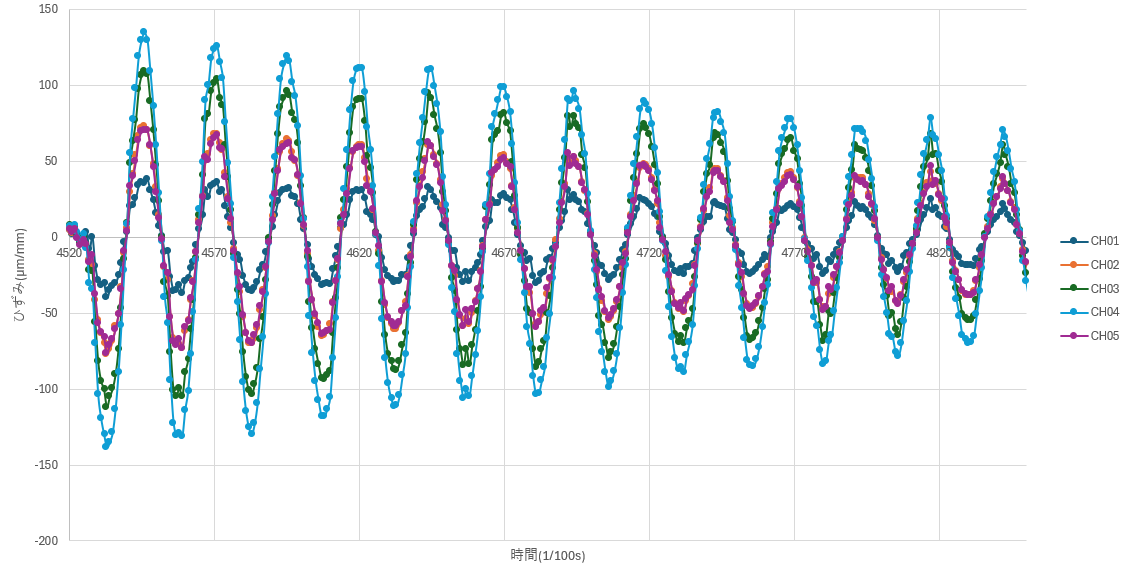
\includegraphics[width=0.8\linewidth]{summer/ship-experiment/bend/picture/hizumi-time-3.png}
    \caption{ひずみ-時間曲線(3回目の打撃に注目)}
    \label{fig:hizumi-time-3}
\end{figure}
さらに細かくみてみると
\begin{figure}[H]
    \centering
    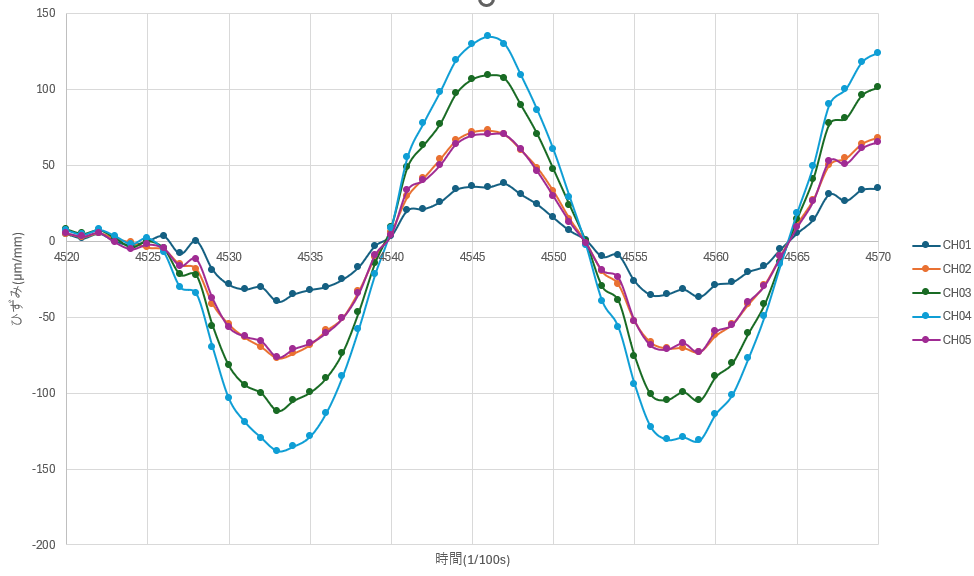
\includegraphics[width=0.5\linewidth]{summer/ship-experiment/bend/picture/hizumi-time-detail.png}
    \caption{ひずみ-時間曲線(さらに3回目の打撃に注目)}
    \label{fig:hizumi-time-detail}
\end{figure}
このように周期的な振動をしていることがわかる。

--

\section{考察}

\subsection{理論値と実験値の比較}
\ref{tex:furoku2}に示された理論式に基づき、荷重-たわみ理論式および荷重-ひずみ理論式を導出した。

それぞれのx座標ごとにみてみると

\begin{figure}[H]
    \centering
    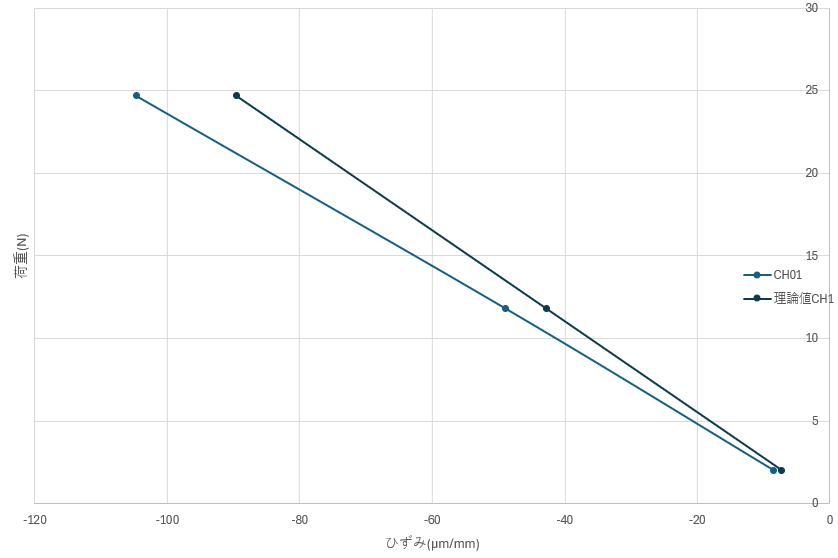
\includegraphics[width=0.8\linewidth]{summer/ship-experiment/bend/picture/ch1.png}
    \caption{荷重-ひずみ曲線(CH1)}
    \label{fig:ch1}
\end{figure}

\begin{figure}[H]
    \centering
    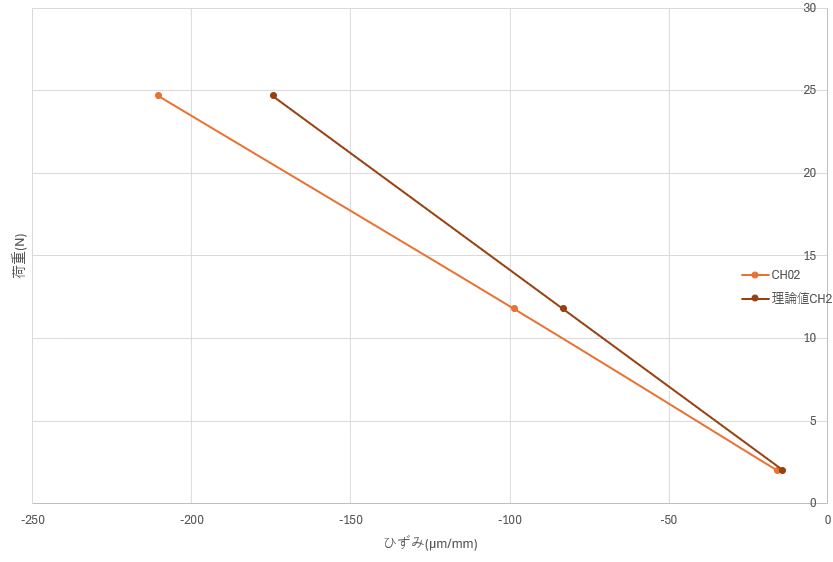
\includegraphics[width=0.8\linewidth]{summer/ship-experiment/bend/picture/ch2.png}
    \caption{荷重-ひずみ曲線(CH2)}
    \label{fig:ch2}
\end{figure}

\begin{figure}[H]
    \centering
    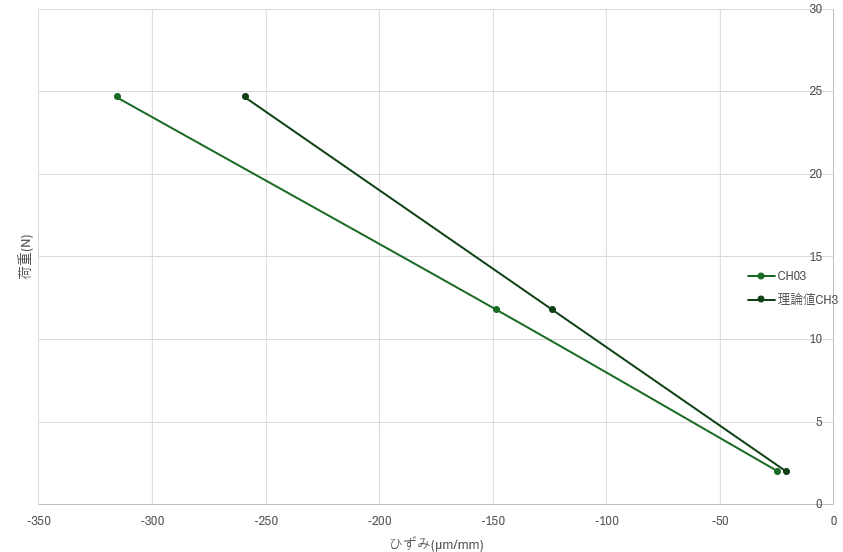
\includegraphics[width=0.8\linewidth]{summer/ship-experiment/bend/picture/ch3.png}
    \caption{荷重-ひずみ曲線(CH3)}
    \label{fig:ch3}
\end{figure}

\begin{figure}[H]
    \centering
    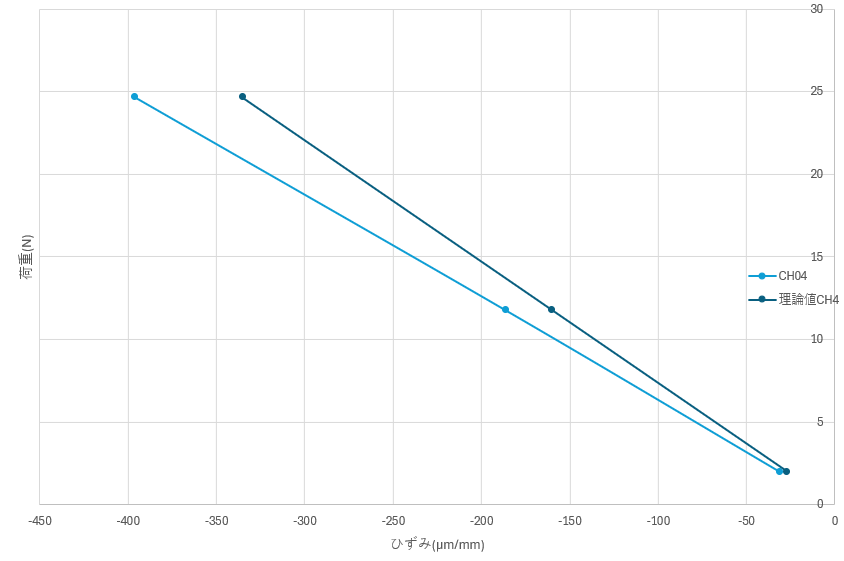
\includegraphics[width=0.8\linewidth]{summer/ship-experiment/bend/picture/ch4.png}
    \caption{荷重-ひずみ曲線(CH4)}
    \label{fig:ch4}
\end{figure}

\begin{figure}[H]
    \centering
    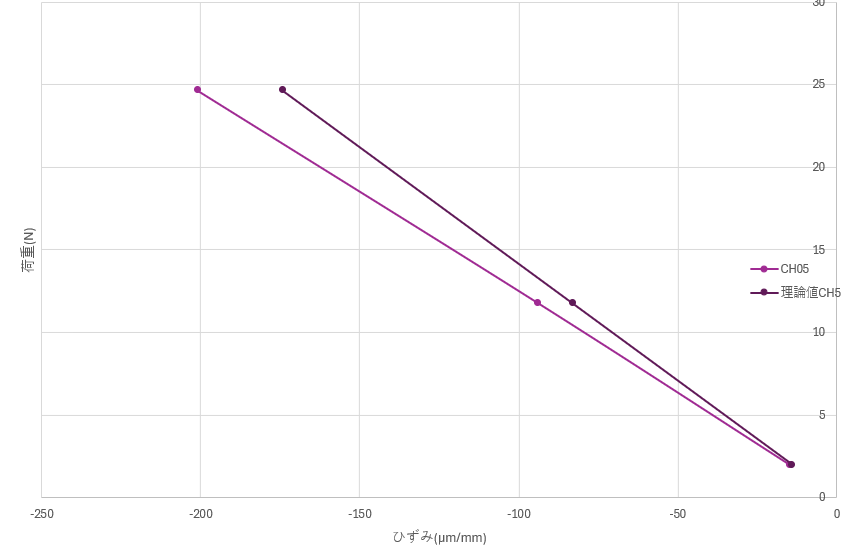
\includegraphics[width=0.8\linewidth]{summer/ship-experiment/bend/picture/ch5.png}
    \caption{荷重-ひずみ曲線(CH5)}
    \label{fig:ch5}
\end{figure}

\begin{figure}[H]
    \centering
    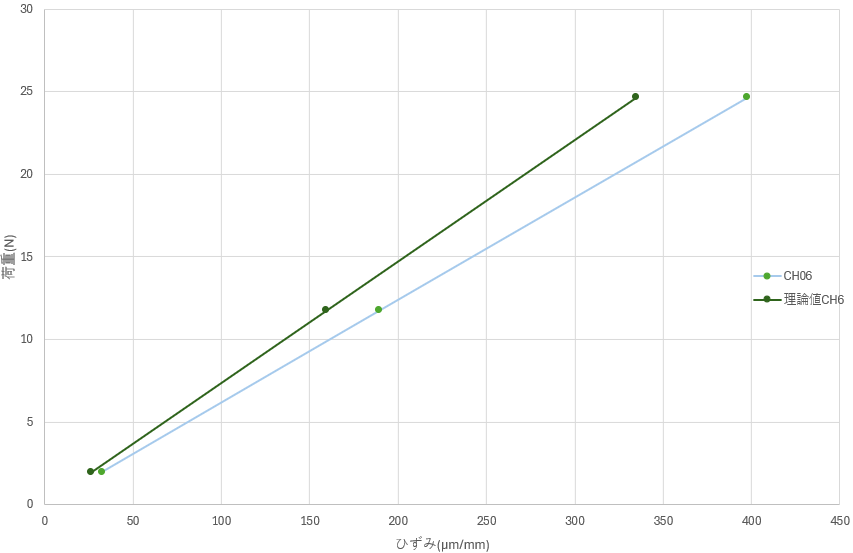
\includegraphics[width=0.8\linewidth]{summer/ship-experiment/bend/picture/ch6.png}
    \caption{荷重-ひずみ曲線(CH6)}
    \label{fig:ch6}
\end{figure}

理論式から導出した理論値と実験値を比較した。図\ref{fig:kaju-hizumi}および図\ref{fig:kaju-tawami}から、本実験において荷重とひずみ、および荷重とたわみの間には、良好な線形関係(比例関係)が見られた。これは、材料が弾性範囲内で変形していることを示唆している。一方で、理論値と実験値にはわずかな乖離が見られた。この乖離は、理論モデルの単純化 (理想的な支持条件の仮定など)や、実験における計測誤差に起因すると考えられる。

\subsection{ヤング率の推定}
実験結果を最もよく説明できるような最適なヤング率を推定した。具体的には、(\ref{eq:3point})式を使ってモーメントを出し、荷重が一定の区間のひずみを抽出し相加平均をとる。そこで、(\ref{eq:strain})式の左辺にひずみの相加平均、右辺の$M$にモーメントを代入してヤング率$E$を得る。という方法を用いた。これをすべての地点について行い。平均をとるという方法で最適なヤング率とした。計算の結果、ヤング率は$E = 1.76 \times 10^5 \ \mathrm{N/mm^2} \ (176 \ \mathrm{GPa})$と推定された。

\subsection{梁の長さ方向にわたるモーメント分布図}
実験で得られたひずみ値から、各測定点における曲げモーメントを算出しプロットした。このモーメント分布は、中央で最大となる三角形の分布に近い形状をしており、理論的な曲げモーメント分布とおおむね一致していることが確認できた。

\begin{figure}[H]
    \centering
    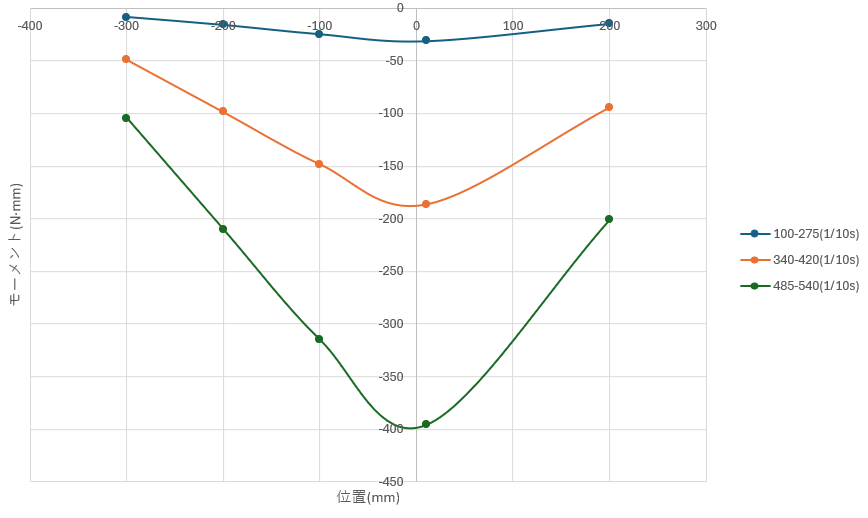
\includegraphics[width=0.5\linewidth]{summer/ship-experiment/bend/picture/moment.png}
    \caption{曲げモーメント図}
    \label{fig:bmd2}
\end{figure}

\subsection{動的過程における固有周期と減衰係数比}
\textbf{固有周期}

図\ref{fig:hizumi-time-detail}のように拡大表示することで1周期における打点の数を数える事を複数回行う事で固有周期を得た。
計算結果は$T=0.25$となった。

\textbf{減衰係数比}

固有周期と同様に拡大表示を行い、振動の最大値、すなわち振幅をそれぞれの山で見つけて、その変遷を観察した。
具体的には$\gamma=\frac{\log{\frac{A_{i}}{A_{i+1}}}}{2\pi}$を用いて複数区間の減衰係数比を算出し、それぞれ相加平均をとった。
計算結果は$\gamma=0.006045$となった。

\subsection{理論式による固有周期の算出}
両端支持梁の理論式を用いて、固有周期の理論値を算出した。断面二次モーメント$I$は、梁の平均寸法(幅$b=24.93 \ \mathrm{mm}$、板厚$h=4.12 \ \mathrm{mm}$)を用いて以下のように計算した。
$$
I = \frac{bh^3}{12} = \frac{24.93 \times (4.12)^3}{12} \approx 145.6 \ \mathrm{mm^4}
$$
これを用いて固有角振動数$\omega$を求め、周期$T_{th}$を算出した。計算には、動的試験で用いた全質量(\ref{tab:weights}で求めたものの総和)$M=2.51kg$、ヤング率$E = 2.06 \times 10^5 \ \mathrm{N/mm^2}$を用いた。
$$
\omega = \sqrt{\frac{48EI}{ML^3}} \quad \text{より} \quad T_{th} = \frac{2\pi}{\omega} \approx 0.21 \ \mathrm{s}
$$
実験値($T = 0.25 \ \mathrm{s}$)は理論値よりやや大きい結果となった。これは、理論式が梁自体の質量を無視していること等が影響していると考えられる。

\subsection{四点曲げのメリット}
本実験で採用した三点曲げに対し、四点曲げは、試験片の中央部において曲げモーメントが一定で、せん断力がゼロの区間を作ることができる。この純粋な曲げ状態により、材料固有の曲げ特性やヤング率をより正確に評価できる点がメリットであると考えられる。
\begin{figure}[H]
    \centering
    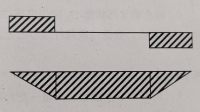
\includegraphics[width=0.5\linewidth]{summer/ship-experiment/bend/picture/4tenmage.png}
    \caption{4点曲げ 剪断応力図, 曲げモーメント図}
    \label{fig:4tenmage}
\end{figure}

\end{document}